% !TEX root = ../main.tex

\chapter{Superradiant scattering of plane waves} % Main chapter title
\label{Chapter5}

The prediction of EM and gravitational radiation amplification was a surprising prediction of Einstein's theory of gravitation in the Kerr geometry.
A method for direct or indirect observation of this process would provide a probe of rotating BHs and thus it would constitute an important test of GR in regions of extreme gravity.
We have studied so far under which conditions an EM mutipole mode $(\omega,\ell, m)$ can undergo superradiant scattering.
We know that each mode will be independently amplified/attenuated as shown above.
The challenge is to observationally infer the occurrence of superradiance for a realistic EM wave, which is generically a superposition of superradiant and non-superradiant modes.

Having shown that superradiance occurs for small frequencies we need to find astrophysical sources that emit EM waves.
Binary systems of rotating neutron stars and BHs may exhibit the necessary conditions for superradiant scattering.
These objects, also known as pulsars, possess a strong magnetic field with magnetic dipole moment typically misaligned with the rotation axis.
Obviously the magnetic field configuration of a neutron star can be very complicated but its main properties are best described by the \emph{oblique-rotator} model, which considers only the leading order in the multipolar expansion, \emph{i.e.} a magnetic dipole moment
\begin{align}
    \mathbf{m}_P = \frac{m_P}{2} \left[ e^{-i \omega t} \sin\alpha_S ( \mathbf{\hat{x}} \pm i \mathbf{\hat{y}}) + \cos\alpha_S \,\mathbf{\hat{z}} \right] + \text{ c.c.} ~,
\end{align}
where $\omega$ is the frequency of rotation.
The upper (lower) sign corresponds to a neutron star co-rotating (counter-rotating) with the BH.
The moment $\mathbf{m}_P$ makes an angle $\alpha_S$ with the rotation axis, resulting in the precession of the pulsars' magnetic axis, which produces a periodic focused beam of EM radiation.
This periodicity is so precise that makes pulsars ideal for measuring time differences in GR tests.
Some neutron stars have a millisecond rotation period producing radiation of a few kHz, which is in range of the superradiant frequencies of a typical stellar mass BH.  

We will focus on scattering of incident plane waves, which means we will consider a source that is far away from the BH.
More specifically, we consider incident plane waves from a magnetic dipole source whose electric and magnetic radiation fields, which are found in standard textbooks, are given by
\begin{align}
    \begin{split}
        \mathbf{E} &= \frac{\mu_0}{8\pi}
        \frac{e^{i\omega|\mathbf{r}-\mathbf{r}_S|}}{|\mathbf{r}-\mathbf{r}_S|} \left(
        \frac{\mathbf{r}-\mathbf{r}_S}{|\mathbf{r}-\mathbf{r}_S|} \times
        \frac{\dd^2 \mathbf{m}_P}{\dd t^2} \right) + \text{ c.c.} \\
        & \simeq  - \frac{\mu_0}{8\pi} \frac{e^{i \omega L}}{L}
        e^{i \mathbf{k} \cdot \mathbf{r}} \left( \mathbf{\hat{r}}_S \times
        \frac{\dd^2 \mathbf{m}_P}{\dd t^2} \right) + \text{ c.c.} ~,
    \end{split}
\end{align}
where $\mathbf{k}= -\omega \mathbf{\hat{r}}_S$ and $L=|\mathbf{r}_S|$ is the distance between the source and the BH.
This approximation is valid when $r=|\mathbf{r}|$ is large compared with the radiation wavelength and the physical dimension of the dipole.
Additionally, in the last step we require that $r \ll L$.
With the similar procedure the magnetic field can be obtain using $\mathbf{B}\simeq - \mathbf{\hat{r}}_S \times \mathbf{E}$.
Thus, when sufficiently far away from the dipole the radiation can be seen as plane waves propagating in the direction of $(- \mathbf{\hat{r}}_S) = (\sin\theta_0 \cos\varphi_0, \sin\theta_0 \sin\varphi_0, \cos\theta_0)$.

%----------------------------------------------------------------------------------------

\section{Harmonics decomposition}

By projecting the complex representation of $\mathbf{E}$ using the perpendicular directions $\mathbf{e}_{\hat{\theta}_0}$ and $\mathbf{e}_{\hat{\varphi}_0}$, we can obtain the two EM field polarizations,
\begin{align}
    \epsilon_{\theta} = \frac{\mu_0 \,m_P \,\omega^2 \sin\alpha_S}{8 \pi} \frac{e^{i \omega L}}{L} e^{\pm i \varphi_0} \cos\varphi_0 ~,\qquad
    \epsilon_{\varphi} = \pm i\, \frac{\mu_0 \,m_P \,\omega^2 \sin\alpha_S}{8 \pi} \frac{e^{i \omega L}}{L} e^{\pm i \varphi_0} ~,
\end{align}
To use results from previous chapters it is convenient to write the EM degrees of freedom using the NP formalism.
There is no need for computing both NP scalars, since we know that the result will be very similar.
Asymptotically we have $\mathfrak{m}\sim \partial_\theta + i \csc\theta \,\partial_\varphi$, thus we may show that $\phi_0 = (\mathbf{E} + i \mathbf{B}) \cdot (\mathbf{e}_{\hat{\theta}} + i \mathbf{e}_{\hat{\varphi}} )/\sqrt{2}$ and $2\phi_2 = (\mathbf{E} + i \mathbf{B}) \cdot (\mathbf{e}_{\hat{\theta}} - i \mathbf{e}_{\hat{\varphi}} )/\sqrt{2}$.
Together with the dipole field approximation, this expansion is valid for $r_{+} \ll r \ll L$.
Following the work done in \cref{Chapter4}, we will keep using $\phi_2$ as our primary scalar as it is the indicated for studying outgoing radiation.
Thus, we may write
\begin{align}
    \label{eq5:phi2plane}
    \phi_2{}^{(\mathrm{plane})} = - \frac{2 \pi i }{3} \left( \epsilon_R \,e^{-i \omega t + i \mathbf{k}\cdot\mathbf{r}} + \epsilon_L^* \,e^{i \omega t - i \mathbf{k}\cdot\mathbf{r}} \right) \sum_{m=-1}^{+1} \uu[-1]{Y}{1,m}(\theta_0,\varphi_0)^{*} \uu[-1]{Y}{1,m}(\theta,\varphi) ~,
\end{align}
where $\mathbf{\hat{k}}\equiv(\theta_0,\varphi_0)$ and $\mathbf{\hat{r}}\equiv(\theta,\varphi)$ are the directions of incidence and observation, respectively.
This result can be easily obtained by explicitly expanding the harmonics sum.
The left and right polarizations are defined as
\begin{align}
    \begin{split}
        \epsilon_R &= \frac{\epsilon_{\theta} - i \epsilon_{\varphi}}{\sqrt{2}}
        = \mp \frac{\mu_0 \,m_P \,\omega^2 \sin\alpha_S}{2\sqrt{6\pi}} 
        \frac{e^{i\omega L}}{L} \,\uu[-1]{Y}{1,\pm 1}(\theta_0,\varphi_0) ~, \\
        \epsilon_L^* &= \frac{\epsilon_{\theta}^* - i \epsilon_{\varphi}^*}{\sqrt{2}} =
        \pm \frac{\mu_0 \,m_P \,\omega^2 \sin\alpha_S}{2\sqrt{6\pi}}
        \frac{e^{-i\omega L}}{L} \,\uu[-1]{Y}{1,\mp 1}(\theta_0,\varphi_0) ~.
    \end{split}
\end{align}

It may seem that $\phi_2$ for a plane wave is approximately describe using only $\ell=1$ harmonics, but we must not forget the angular dependence in
\begin{align}
    e^{i \mathbf{k} \cdot \mathbf{r}} = 4 \pi \sum_{\ell,m} i^\ell j_\ell(\omega r) \uu{Y}{\ell m}(\theta_0,\varphi_0)^{*} \uu{Y}{\ell m}(\theta,\varphi) ~,
\end{align}
whose decomposition in terms of $s=0$ spherical harmonics is well-known \cite{Jackson1998}, where $j_\ell(z)$ corresponds to the spherical Bessel function of the first kind.
Substituting this expansion into \eqref{eq5:phi2plane} we obtain a superposition of different spin-weight harmonics and after grouping $\mathbf{\hat{k}}$ and $\mathbf{\hat{r}}$ terms these can be expanded using Clebsh-Gordon coefficients.
\begin{align}
    \label{eq5:phi2planeExpanded}
    \begin{split}
        \phi_2{}^{(\mathrm{plane})} &= - 2 \pi \,\epsilon_R \,e^{-i \omega t} \,\sum_{\ell,m} \left(
        \sum_{n=\ell-1}^{\ell+1} i^{n + 1} \,j_n(\omega r) \,\frac{2n + 1}{2\ell + 1} 
        \left|\langle n,0 ; 1,1 | \ell,1 \rangle\right|^2 \right)
        \uu[-1]{Y}{\ell m}(\mathbf{\hat{k}})^{*} \uu[-1]{Y}{\ell m}(\mathbf{\hat{r}}) \\
        & \qquad + ( \,\epsilon_R \to \epsilon_L^*, \,\omega \to -\omega \,) \\[0.15cm]
        &\sim + 2 \pi \,\epsilon_R \,e^{-i \omega t} \,\sum_{\ell,m} \left(
        -\frac{1}{2 \omega} \frac{e^{i \omega r}}{r} 
        + (-1)^\ell \,\frac{\ell(\ell+1)}{8 \omega^3} \frac{e^{-i \omega r}}{r^3} \right)
        \uu[-1]{Y}{\ell m}(\mathbf{\hat{k}})^{*} \uu[-1]{Y}{\ell m}(\mathbf{\hat{r}}) \\
        & \qquad + (\,\epsilon_R \to \epsilon_L^*, \,\omega \to -\omega \,) ~.
    \end{split}
\end{align}
The expression for $\phi_0$ is very similar, changing the coefficients of $e^{\pm i \omega r}$ accordingly so they obey Eqs. \eref{eq3:separationB} and \eref{eq3:separationBdagger} when $r \gg r_{+}$, replacing $\uu[-1]{Y}{\ell m}(\mathbf{\hat{r}})\to\uu[+1]{Y}{\ell m}(\mathbf{\hat{r}})$.

We have shown that even a simple plane wave is a superposition of modes with positive and negative frequencies modulated by the left and right polarizations, respectively, which are proportional to $\uu[-1]{Y}{1, \pm 1}(\theta_0, \varphi_0)$.
According to condition \eref{eq3:superradiance}, modes with either $\omega>0$, $m>0$ or $\omega<0$, $m<0$ can be amplified.
The position of the source modulates the incident wave changing its mode composition. 
Therefore if the plane wave source co-rotates with the BH, when $\theta_0 \to 0$ the positive frequencies dominate because $\epsilon_L^*\to 0$, coinciding with the region were $m>0$ harmonics predominate. Analogously, when $\theta_0\to\pi$ negative frequencies dominate as $\epsilon_R \to 0$.
On the other hand, when considering counter-rotation and the incidence at one of the poles, harmonics with $m \omega >0$ have null coefficients so those modes are never amplified.
More specifically, when we have exactly $\theta_0=0$ ($\theta_0=\pi$) the modes $m=1$ ($m=-1$) are the only non-zero contributions of the EM wave if and only if the source co-rotates with the BH, while other $m$ modes vanish.
This has been used in \cite{Rosa2016} to show that a plane wave can be overall amplified by a spinning black hole when it is incident along the BH rotation axis and the source co-rotates with the latter. For a pulsar orbiting a Kerr BH, this results in a modulation of the pulsar’s total luminosity.

%----------------------------------------------------------------------------------------

\section{Scattering theory}

We understand that we(US HUMANS) have limited observational capabilities and only have access to given a direction of observation for this hypothetical binary system.
If it were possible to map the entire scattered wave with enough detail we could in principle extract and compare each mode with the ones of the emitted wave. For this analysis we would only need to know the global gain/loss factor, given by $\uu[\pm1]Z{\ell m}$. Therefore we will resort to scattering theory of waves to study the angular effects of superradiance.

Intuitively, it is understood that only a small part of the incident wave will be scattered by the BH.
The scattered part together with the indent wave produce a characteristic interference pattern.
In order to differentiate the scattered wave we need to remove the background incident plane wave.
Scattering theory assumes that we may write
\begin{align}
    \label{eq5:scattering}
    \phi_2 - \phi_2{}^{(\mathrm{plane})} = f(\theta,\varphi) \frac{e^{i \omega (r_{*}-t)}}{r} + (\omega\to-\omega, \,f \to g) ~,
\end{align}
where $\phi_2$ is written similarly with coefficients $\mathscr{Z}_\mathrm{out}$ and $\mathscr{Z}_\mathrm{in}$ obtained numerically in \cref{Chapter4}.

Up to this point we used the approximation of plane wave first introduced in \eref{eq5:phi2plane}, which can only be used in flat space. The fact is that this approximation does not take into account the long-range behaviour of Kerr's gravitational field, which decays as $\mathscr{O}(\tfrac{1}{r})$ as obtained in \eref{eq3:asymptoticVeff}.
We know that from the asymptotic form of the radial function that this can be bypassed by a logarithmic phase-correction in the exponential, substituting $r\to r_{*}$.
The ingoing part of $\phi_2$ is naturally the same as $\phi_2{}^{(\mathrm{plane})}$, so that the scattered wave only has an outgoing part, given by
\begin{align}
    \label{eq5:scatterFexpressionYY}
    f(\theta,\varphi) = - \frac{\pi \,\epsilon_R}{\omega} \sum_{\ell,m} \left[
    (-1)^{\ell+1} \frac{\ell(\ell+1)}{4 \omega^2 }
    \frac{\mathscr{Z}_\mathrm{out}}{\mathscr{Z}_\mathrm{in}} - 1 \right]
    \uu[-1]{Y}{\ell m}(\mathbf{\hat{k}})^{*} \uu[-1]{Y}{\ell m}(\mathbf{\hat{r}}) ~.
\end{align}
A similar expression is obtained for $g(\theta,\varphi)$ proportional to $\epsilon_L^*$.

The long-range effect of the background is independent of the BH rotation (also in Schwarzschild), \emph{i.e.} we must not mistake the spherical approximation with long-range effects of the effective gravitational potential.
The plane wave decomposition in \eref{eq5:phi2plane} discards, to a first approximation, the effects of the BH rotation, therefore using spherical rather than spheroidal harmonics.
We nevertheless expect this to be a good first approximation for the small $c$ values relevant for the lowest multipoles in the superradiant frequency regime.
We can also recall that the mode factor in \eqref{eq5:scatterFexpressionYY} is very similar to the expression \eref{eq3:amplificationBAoutAin}, derived in \cref{Chapter3}.
We see that for $a\omega \to 0$,
\begin{align}
    \label{eq5:phaseFactor}
    \frac{\mathscr{B}}{4 \omega^2} \frac{\mathscr{Z}_\mathrm{out}}{\mathscr{Z}_\mathrm{in}} \simeq \frac{\ell(\ell+1)}{4 \omega^2} \frac{\mathscr{Z}_\mathrm{out}}{\mathscr{Z}_\mathrm{in}} ~,
\end{align}
remembering that $\mathscr{B} = \left[ (\uu[\pm 1]{\mathscr{E}}{\ell m})^2 - 4 a^2 \omega^2 + 4 m a \omega \right]^{1/2}$.
An argument could be made that the latter expression for the coefficient is the correct one instead of the one in \eqref{eq5:scatterFexpressionYY}, but this approximation is good enough when considering superradiant frequencies $|\omega| \simeq 0.4 \Omega_H$ for a typical stellar mass extremal BH (see \fref{fig4:plotSWSH12}).

%----------------------------------------------------------------------------------------

\section{Phase shifts}

If wo assume co-rotation of the source with incidence along the axis at $\theta_0=\varphi_0=0$ we will only need to compute $f(\theta,\varphi)$, since $\epsilon_L^*=0$.
This assumption eases the need to compute modes other than $m=1$.
Therefore, truncating the harmonic expansion \eref{eq5:scatterFexpressionYY} at some $\ell=\ell_{\max}$ implies that scattering with incidence on axis reduces the number of necessary harmonics in $\ell_{\max}(\ell_{\max} + 1)$.

Proceeding with the sum over multipoles, using the numerically obtained results for the ratio $\mathscr{Z}_\mathrm{out}/\mathscr{Z}_\mathrm{out}$ as described in the previous chapter, it appears that the partial wave sum is divergent near $\theta = 0$, since the value of increasing $f(0,0)$ seams to increase more with each contribution (see \fref{fig5:sumF}).
\begin{figure}[h]
	\centering
	\vspace{0.2cm}
	\begin{subfigure}[c]{0.6\textwidth}
        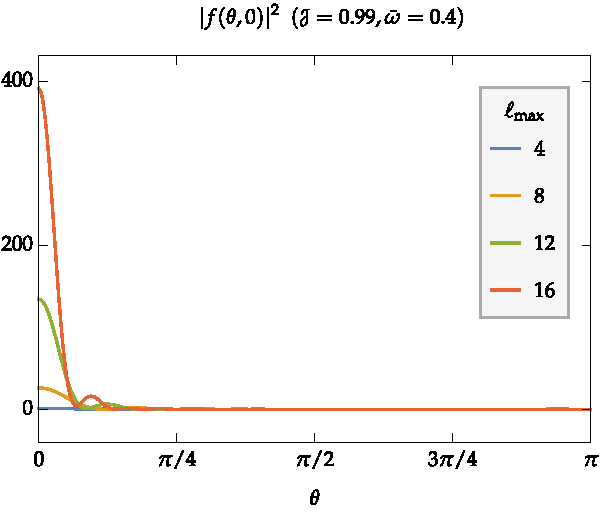
\includegraphics[width=\textwidth]{sumF2}
	\end{subfigure}
	\caption{Eigenvalues for $\ell=1$ (left) and $\ell=2$ (right) for typical values of $c$, using the spectral method.}
	\label{fig5:sumF}
\end{figure}
This problem is due to the long-range effect of the gravitational potential of BHs. Central potentials falling as $1/r$ (check \eref{eq3:asymptoticVeff}) do not have an effect on the global amplitude of the wave but the scattered wave has phase shifts in each of the mode coefficients, producing a divergence at $(\theta,\varphi)=(\theta_0,\varphi_0)$.
This problem was also studied in classical Coloumb scattering, where $f(\theta,0)$ is known to diverge at $\theta=\theta_0$.
This result appears strange at first, but we must remember that, being a complete space of functions, the harmonics obey $\sum_{\ell m} \uu[-1]{Y}{\ell m}(\mathbf{\hat{k}})^{*} \uu[-1]{Y}{\ell m}(\mathbf{\hat{r}})) = \delta(\cos\theta - \cos\theta_0) \delta(\varphi - \varphi_0)$.

In order to regularize the sum for $f(\theta,\varphi)$, it is convenient to separate it in two terms,
\begin{align}
    \label{eq5:fNfD}
    f(\theta,\varphi) = f_\mathrm{N}(\theta,\varphi) + f_\mathrm{D}(\theta,\varphi) ~,
\end{align}
$f_\mathrm{N}(\theta,\varphi)$ carries all the scattering information about the Newtonian effects of the long-range $1/r$ (Coulomb) potential.
It can be written as
\begin{align}
    f_\mathrm{N}(\theta,\varphi) = - \frac{\pi \,\epsilon_R}{\omega}
    \sum_{\ell,m} \left( e^{2 i \delta_N } - 1 \right)
    \uu[-1]{Y}{\ell m}(\mathbf{\hat{k}})^{*} \uu[-1]{Y}{\ell m}(\mathbf{\hat{r}}) ~,
\end{align}
where the phase shifts are \cite{Futterman1988}
\begin{align}
    \label{eq5:phaseShiftN}
    e^{2 i \delta_N } = \frac{\Gamma(\ell + 1 - 2 i M \omega)}{\Gamma(\ell+1 + 2 i M \omega)} ~.
\end{align}
Assuming an incidence $\theta_0=0$, summing the series leads to a similar result as the Rutherford elastic scattering in a Coulomb potential, $|f_\mathrm{N}(\theta,0)|^2 \sim 1/\sin^{4}(\theta/2) \sim 1/\theta^4$, which appears to explain the divergence at $\theta=0$. 

On the other hand, the $f_\mathrm{D}(\theta,\varphi)$ encloses all the information regarding the main scattering effects, including superradiance.
From \eqref{eq5:fNfD}, simple algebra states that
\begin{align}
    \label{eq5:fD}
    f_\mathrm{D}(\theta,\varphi) = - \frac{\pi \,\epsilon_R}{\omega}
    \sum_{\ell,m} \left[ \frac{\mathscr{B}}{\ell(\ell+1)} \sqrt{ \uu[\pm 1]{Z}{\ell m} +1 } \,e^{2 i \delta_\ell } - e^{2 i \delta_\mathrm{N} } \right]
    \uu[-1]{Y}{\ell m}(\mathbf{\hat{k}})^{*} \uu[-1]{Y}{\ell m}(\mathbf{\hat{r}}) ~,
\end{align}
where we define
\begin{align}
    \label{eq5:phaseShiftD}
    2 \delta_\ell = \mathrm{arg} \left[ (-1)^{\ell+1} \,\frac{\mathscr{Z}_\mathrm{out}}{\mathscr{Z}_\mathrm{in}} \right] ~.
\end{align}
For this sum to converge two things must occur.
First, absolute value \eref{eq5:phaseFactor} must go to $1$.
Numerically, we find that in the limit of $\ell/\omega\to \infty$ mode amplitudes are not significantly affected by the BH, $\uu[\pm 1]{Z}{\ell m}\to 0$ (check \fref{fig4:logZ}).
Also, from \eqref{eq3:Bdefinition} we know that for $c=a\omega$ constant, increasing $\ell$ leads to the eigenvalue $\uu[\pm 1]{\mathscr{E}}{\ell m} \sim \ell(\ell+1)$, which cancels the factor in \eref{eq5:fD}.

Secondly, the numerically computed phases using \eref{eq5:phaseShiftD} must converge to the Newtonian phase shifts \eref{eq5:phaseShiftN}, $\delta_\ell \to\delta_N$.
Results appear to indicate that these phases, like $\delta_N$, are independent of $m$.
Also they appear to have the same asymptotic form, apart from a constant offset $\delta_0$. 
We attribute this difference to an ambiguity in the definition of the tortoise coordinate, given by
\begin{align}
    r_{*} = r +  \frac{2M r_{+}}{r_{+}-r_{-}} \log\left( \frac{r-r_{+}}{r_{+}}\right) -   \frac{2M r_{-}}{r_{+}-r_{-}} \log\left( \frac{r-r_{-}}{r_{-}} \right) + \text{ const. } ~,
\end{align}
which is needed to extract the complex asymptotic coefficients of \eref{eq3:asymptoticR}.
\begin{figure}[h]
	\centering
	\vspace{0.2cm}
	\begin{subfigure}[c]{0.49\textwidth}
        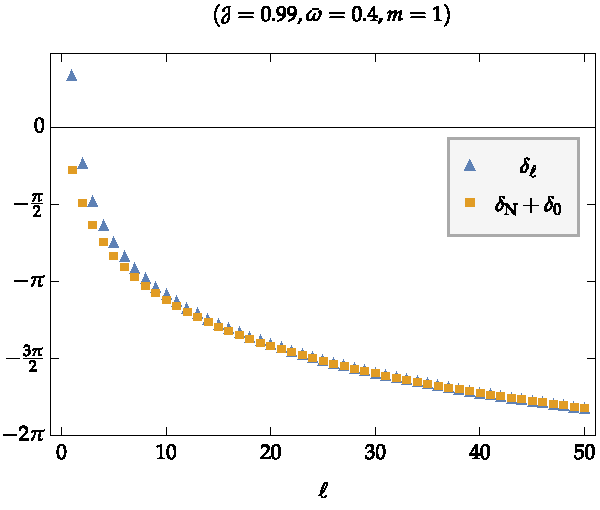
\includegraphics[width=\textwidth]{arg2}
    \end{subfigure}
    \hfill
    \begin{subfigure}[c]{0.48\textwidth}
        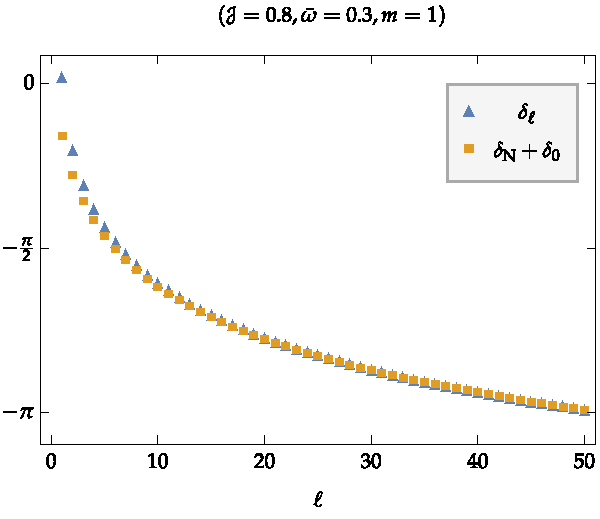
\includegraphics[width=\textwidth]{arg3}
    \end{subfigure}
    \hfill
	\caption{Eigenvalues for $\ell=1$ (left) and $\ell=2$ (right) for typical values of $c$, using the spectral method.}
	\label{fig5:argZoutZin}
\end{figure}
It is expect for this integration constant to be dependent only on $a$ and $M$, which implies that for constant $\bar{\omega}$ the value of $\delta_0$ depends only on $\mathscr{J}$.
We fit numerically the value of $\delta_0$ independently for each case.
From \fref{fig5:argZoutZin} we verify that these phases indeed share the same asymptotic behaviour when $\ell\gg 1$.
On the other hand, larger deviations from the $\delta_N$ occur for values of $\ell$ close to $1$ where effect BH spin are predominant.
Taking the $\mathscr{J} \to 0$ limit quickly takes the values of $\delta_\ell$ closer to $\delta_N$.

The correspondent partial wave sums for the phases presented above are shown in \fref{fig5:fD}.
The truncation of the series \eref{eq5:fD} at $\ell=\ell_\mathrm{max}$ leads to interference oscillations of characteristic length $2\pi/\ell_\mathrm{max}$.
Comparing with \fref{fig5:sumF} it seams that the partial wave expansion for $|f_\mathrm{D}(\theta,0)|^2$ is now converging in the range $32 \le \ell_\mathrm{max} \le 48$.
We expected that the computation of $f_D(\theta, \varphi)$ would give us a clean channel to identify superradiance phenomena in scattering of plane waves, but \fref{fig5:fD} shows that performing the mode sum from $\ell=16$ through $\ell=24$, which we know to have effectively $\uu[\pm 1]{Z}{\ell 1}=0$ ($<10^{-85}$), still has a great impact on the value of $|f_D(\theta,0)|^2$.
Even tough these modes are fully reflected, effects of amplification/absorption are masked by the mode interference introduced by the phase shifts in each mode.
Thus we must find other ways of isolating these effects from relevant superradiant modes with lower $\ell$ values.
\begin{figure}[h]
	\centering
	\vspace{0.2cm}
	\begin{subfigure}[c]{0.49\textwidth}
        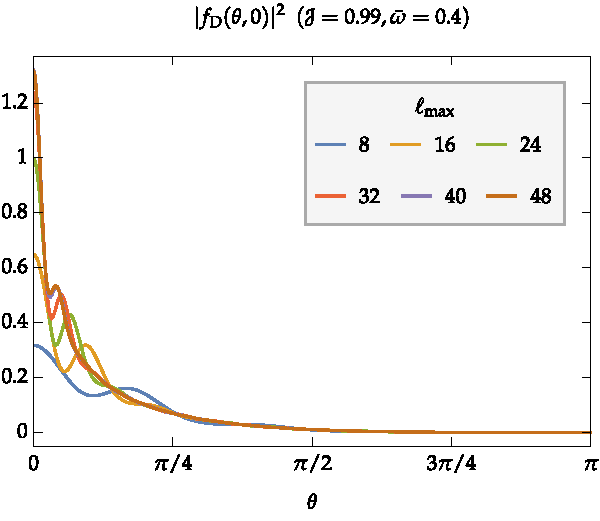
\includegraphics[width=\textwidth]{sumFD2}
    \end{subfigure}
    \hfill
    \begin{subfigure}[c]{0.48\textwidth}
        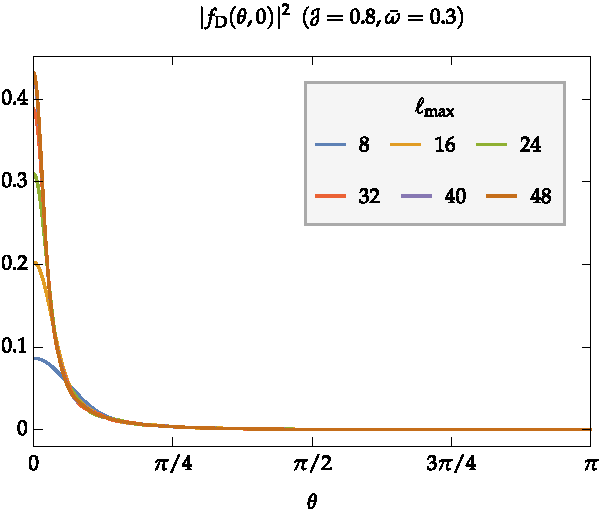
\includegraphics[width=\textwidth]{sumFD3}
    \end{subfigure}
    \hfill
	\caption{Eigenvalues for $\ell=1$ (left) and $\ell=2$ (right) for typical values of $c$, using the spectral method.}
	\label{fig5:fD}
\end{figure}

\cleardoublepage